\documentclass[12pt, oneside]{extbook}
\usepackage[utf8]{inputenc}
\usepackage[russianb]{babel}
\newtheorem{theorem}{\protect\thmname}
\newcommand{\thmname}{}\newcommand{\exaname}{} % initialization
\addto\captionsrussian{
  \renewcommand{\thmname}{Теорема}
}
\usepackage{vmargin}
\setpapersize{A4}
\setmarginsrb{30mm}{20mm}{15mm}{20mm}{0pt}{0mm}{0pt}{13mm}
\usepackage{indentfirst}
\usepackage{setspace}
\setstretch{1.5}
\sloppy
\usepackage{graphicx}
\usepackage{amsfonts}
\graphicspath{ {./pics/} }
\usepackage{subfig}

\begin{document}
\pagenumbering{gobble}
\begin{figure}[h]

\includegraphics{MB}
\centering
\end{figure}
\center{
Московский государственный университет имени М.В. Ломоносова\\
Факультет вычислительной математики и кибернетики\\
Кафедра нелинейных динамических систем и процессов управления\\
}
\vspace*{3\baselineskip}
\center{
{\large Сивков Антон Александрович}\\
\medskip
{\Large \textbf{Применение нейроных сетей для моделирования систем управления}}\\
\vspace*{3\baselineskip}
ВЫПУСКНАЯ КВАЛИФИКАЦИОННАЯ РАБОТА\\
}
\vspace*{4\baselineskip}
{\flushright
\textbf{
Научный руководитель:
}\\
д.ф-м.н., профессор\\
В. В. Фомичев\\
}
\vfill
\center{Москва, \the\year}
\clearpage
\pagenumbering{arabic}
\pagestyle{plain}
\setcounter{page}{2}
\tableofcontents
\begin{flushleft} \setlength{\parindent}{1cm}
\chapter{Введение}
\section{Постановка задачи}
Данная работа ставит целью сравнительный анализ способности нейронных сетей с различными архитектурами аппроксимировать объекты управления для задач идентификации, основное сравнение происходит в контексте способности сетей экстраполировать поведение объектов управления. Попытка экстраполяции поведения не всегда корректна с математической точки зрения, однако экстраполирование позволяет сравнивать качество идентификации систем управления, не прибегая к моделированию сложных нелинейных систем.
\section{Виды идентификации}
В теории управления одной из основных задач является задача идентификации систем, задача построения математической модели объекта управления, способной адекватно воспроизводить реальное поведение объекта управления.
\par
Задачи идентификации приблизительно можно разделить на 3 вида:\\
\begin{itemize}
\item Модель 'белого ящика', модель применяется, когда точно известен основополагающий принцип, лежащий в основе устройства системы. Модель может применятся например для систем, описывающих взаимодействия в рамках законов Ньютона. Зачастую такие системы имеют сложную структуру, и для построения точной модели требуются неадекватные затраты времени.
\item Модель 'серого ящика', модель применяется, когда известны или имеются достачно сильные предположения о характере соотношений между входом и выходом системы, но остается некоторое количество 'свободных' параметров системы, которые приближаются с использованием данных выходов и входов системы. Модель может применятся, например для приближения параметров уравнения Моно при моделировании микробных популяций.
\item Модель 'чёрного ящика', модель применяется, когда сложно сделать какие-либо априорные предположения о структуре системы, в этой модели используются только данные о входах и выходах системы, модель применяется к различным нелинейным системам. В этой работе используется эта модель, нейронные сети обучаются моделировать 'черный ящик'. 
\end{itemize}
\par
Сама идея применения неронных сетей для моделирования объектов управления не нова, примеры можно найти в публикации \cite{fc90}, датированной 1990 годом, где простейшие сети используются для моделирования простых дискретных линейных объектов управления.
\par 
Хотя для простейших архитектур нейронных сетей сходимость доказуема, множество современных архитектур нейросетей не имеют под собой теоретической базы, котороя обосновывала бы их сходимость, тем не менее, они сходятся, и показывают впечатляющие результаты в задачах обработки речи, изображений, естественных языков, и многих других.\\
\section{Объект управления, использованный для экспериментов}
Для экспериментов использовался простейший объект управления, который можно описать следующей дискретной передаточной функцией:\\
\begin{equation} \label{eq:1}
H = \frac{z}{(z-\frac{1}{2})(z-\frac{1}{3})(z-\frac{1}{4})}
\end{equation}
\par
Объект устойчив, в экспериментах $dt = 1~sec$. Выглядит нелогичным проведение экспериментов, которые имеют смысл для сложных нелинейных объектов, на простейшем линейном дискретном объекте, однако данная работа имеет цель провести сравнительный анализ различных архитектур нейронных сетей, и, как показывает практика, даже такой простой объект позволяет сделать однозначные выводы относительно преимуществ одной архитектуры над другой.
\chapter{Моделирование с помощью многослойного перцептрона}
\section{Структура сети}
Многослойный перцептрон получил слово 'перцептрон' в названии в силу исторических причин, и его структура существенно отличается от структуры перцептрона Розенблатта, прежде всего тем, что он может иметь сколь угодно много слоев, и иметь обучаемые веса в каждом слое.
\begin{figure}[h]
\centering
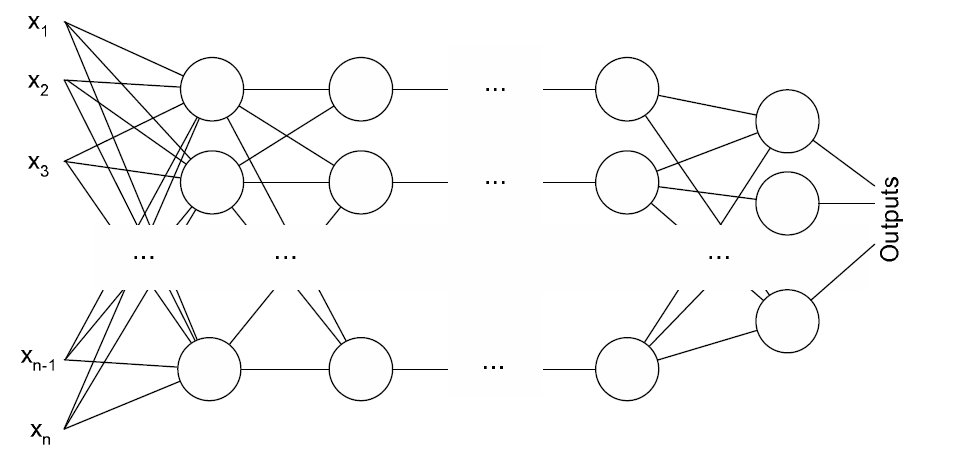
\includegraphics[width=0.5\textwidth]{multi_layer_perceptron_general}
\caption{Многослойный перцептрон.}
\label{fig:multi_perceptron}
\end{figure}
\par
Устройство перцептрона схематично представлено на рисунке \ref{fig:multi_perceptron}, $x_i$ обозначает i-й вход сети. Каждый из обозначенных на рисунке узлов сети выполняет следующее преобразование: $y = f(<w, x> + b)$, т. е. функция активации $f$ (как правило сигмоида, тангенс или ReLu), примененная к скалярному произведению вектора входов узла $x$ на вектор весов узла $w$ плюс сдвиг $b$ (bias). При обучении сети с помощью стохастического градиентного спуска веса изменяются на каждой итерации в направлении антиградиента функции ошибки предсказания сети $L(x, y, w)$ на текущих данных. Значение градиента вычисляется с помощью метода \textit{обратного распространения ошибки}. Этот метод вкратце можно описать так:\\
Пусть дан некий узел сети, для удобства отбросим функцию активации, т.к. она не влияет существенно на принцип вычислений. Пусть $y$ --- выход узла, $w_{i}$ --- веса узла, $x_{i}$ --- входы $i=1,...,n$, тогда справедливы следующие формулы:\\
\begin{equation} \label {eq:2}
\frac{\partial L}{\partial w_{i}} = \frac{\partial L}{\partial y} * \frac{\partial y}{\partial w_{i}} = \frac{\partial L}{\partial y} * x_{i}
\end{equation}\\
\begin{equation} \label {eq:3}
\frac{\partial L}{\partial x_{i}} = \frac{\partial L}{\partial y} * \frac{\partial y}{\partial x_{i}} = \frac{\partial L}{\partial y} * w_{i}
\end{equation}\\
Формула \ref{eq:2} позволяет вычислить производную ошибки по конкретному весу сети, если известна производная ошибки по выходу узла $\frac{\partial L}{\partial y}$, а формула \ref{eq:3} позволяет вычислить производную ошибки по выходам узлов, не являющихся выходными, путем рекурсивного рассчета производных по выходам, при этом рассчет происходит от выходов сети ко входам, в направлении, \textit{обратном} прямому вычислению.
\section{Код и схема модели}
\begin{figure}[h]
\centering
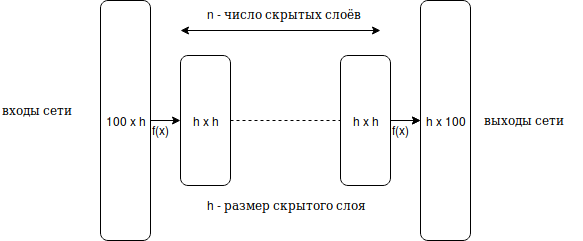
\includegraphics[width=0.9\textwidth]{multi_layer_perceptron}
\caption{Использованная для экспериментов архитектура}
\label{fig:my_multi_perceptron}
\end{figure}
Один из вариантов многослойного перцептрона, использованного для моделирования объекта управления \ref{eq:1} изображен на рисунке \ref{fig:my_multi_perceptron}. Гиперпараметры сети: число скрытых слоёв n; размер скрытого слоя h; функция активации f(x). Такой перцептрон может быть реализован на языке python с помощью библиотеки pytorch \footnote{код всех моделей и jupyter notebook с экспериментами можно найти в \cite{source_code}}:
\begin{verbatim}
class MultiPercNet(nn.Module):

    def __init__(self, input_size, output_size, n_layers, layer_size):
        super().__init__()
        self.layers = nn.ModuleList([nn.Linear(input_size, layer_size)])
        self.layers.extend(nn.Linear(layer_size, layer_size) for _ in range(n_layers - 2))
        self.layers.append(nn.Linear(layer_size, output_size))
        self.layer_size = layer_size
        for layer in self.layers:
            nn.init.xavier_uniform_(layer.weight, gain=1)
        self.input_size = input_size
        self.layer_size = layer_size
        self.tanh = nn.Hardtanh(min_val=-1, max_val=1)

    def forward(self, x):
        y = self.tanh(self.layers[0](x))
        for i in range(1, len(self.layers)):
            y = self.tanh(self.layers[i](y))
        return y
\end{verbatim}
\par
Сеть обучалась с использованием среднеквадратичной ошибки в качестве функции ошибки.
\pagebreak
\section{Эксперименты}
\begin{figure}[h]
\centering
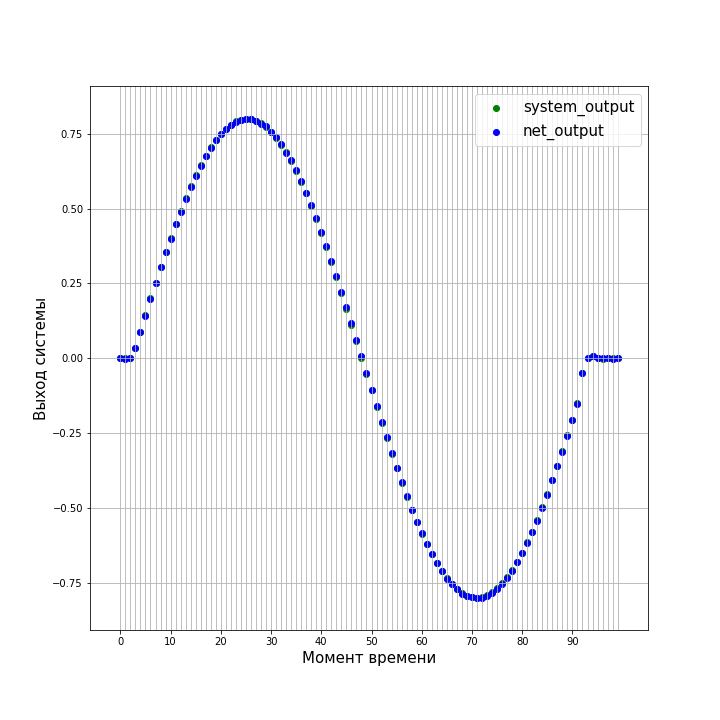
\includegraphics[width=0.9\textwidth]{fcnet_prediction}
\caption{Предсказание при отсутствии сдвига частот.}
\label{fig:multi_prediction}
\end{figure}
Во всех экспериментах сеть обучается на множестве входных и выходных сигналов системы, полученном при подаче на вход системы сигналов со случайной частотой, взятой из равномерного распределния на отрезке [0.05~Гц, 0.1~Гц], входные и выходные сигналы берутся за первые 100 секунд. На рисунке \ref{fig:multi_prediction} показано предсказание и реальный выход системы при подаче на вход системы сигнала со случайной частотой, полученной аналогично частоте входных сигналов, использованных при обучении. Среднеквадратичная ошибка при отсутсвии сдвига частот: 
$ 1.1196042208666767e-05$. Нетрудно заметить, что сеть предсказывает выход объекта управления практически идеально при сохранении той же частоты входных сигналов, что использовалась при обучении. Это объясняется тем, что объект управления имеет простейшую структуру, и сеть без проблем аппроксимирует выходной сигнал объекта управления при подаче входных сигналов, не выходящих за область данных, использованных для обучения.
\par
\begin{figure}[h]
\centering
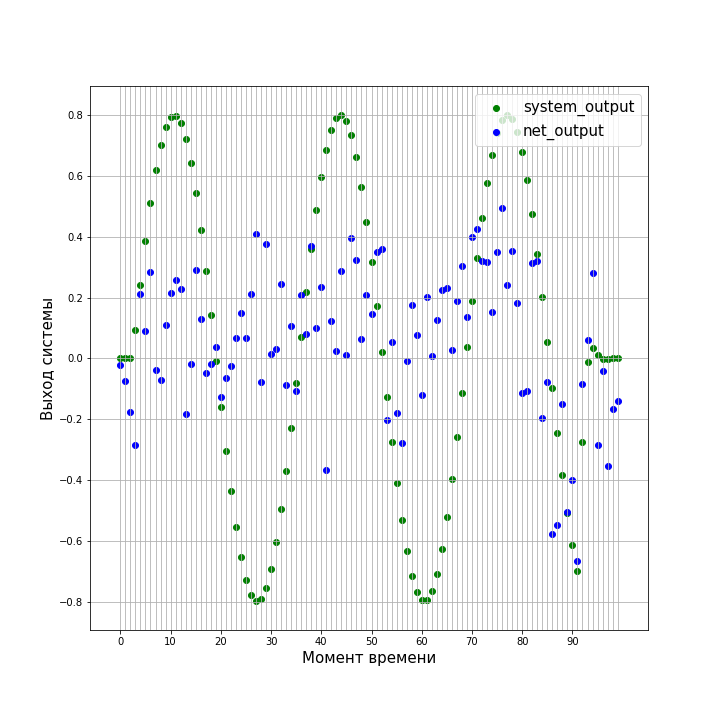
\includegraphics[width=0.9\textwidth]{fcnet_prediction_shifted}
\caption{Предсказание при частоте 0.2~Гц.}
\label{fig:multi_prediction_shifted}
\end{figure}

На рисунке \ref{fig:multi_prediction_shifted} изображено предсказание выхода системы сетью, обученной на входных и выходных данных, полученных при подаче на вход системы сигналов из того же диапазона частот [0.05~Гц, 0.1~Гц], при подаче на вход сигнала с частотой 0.2~Гц. Среднеквадратичная ошибка при подаче сигналов со случайной частотой из равномерного распределения [0.1~Гц, 0.2~Гц]: $ 0.19516661121453216$. Из показателей и рисунка \ref{fig:multi_prediction_shifted} можно сделать вывод о том что сеть не способна предсказать в какой--либо степени релевантные данных при выходе частоты входного сигнала за пределы параметров обучающей выборки. Это также позволяет сделать вывод о том, что сеть переобучается на данных обучающей выборки, и теряет способность к какой--либо экстраполяции поведения объекта управления. 
\par
\begin{figure}[!ht]
     \subfloat[Перебор размера скрытого слоя сети]{
         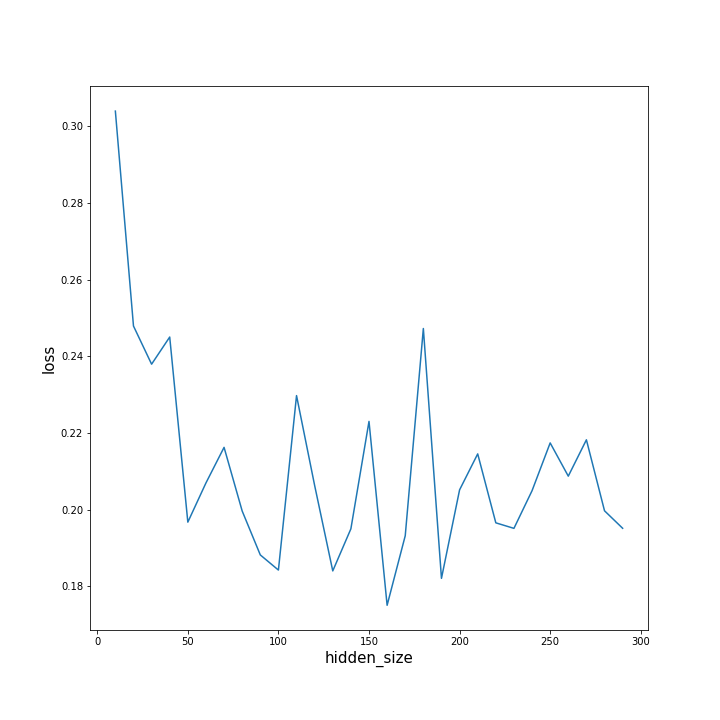
\includegraphics[width=0.45\textwidth]{perceptron_hiddden_size_search}
     }
     \hfill
     \subfloat[Перебор количества внутренних слоев]{
         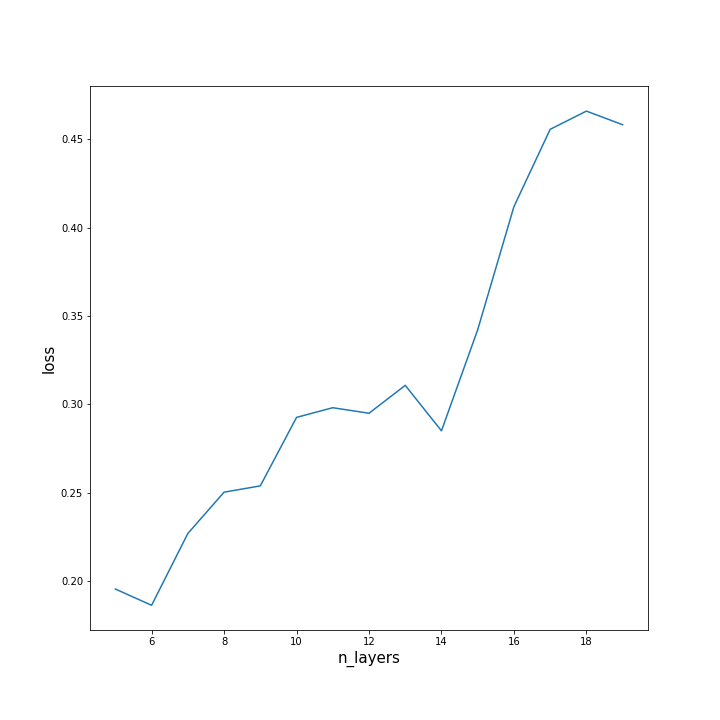
\includegraphics[width=0.45\textwidth]{perceptron_n_layers_search}
     }
     \centering
     \subfloat[Перебор функций активации]{
         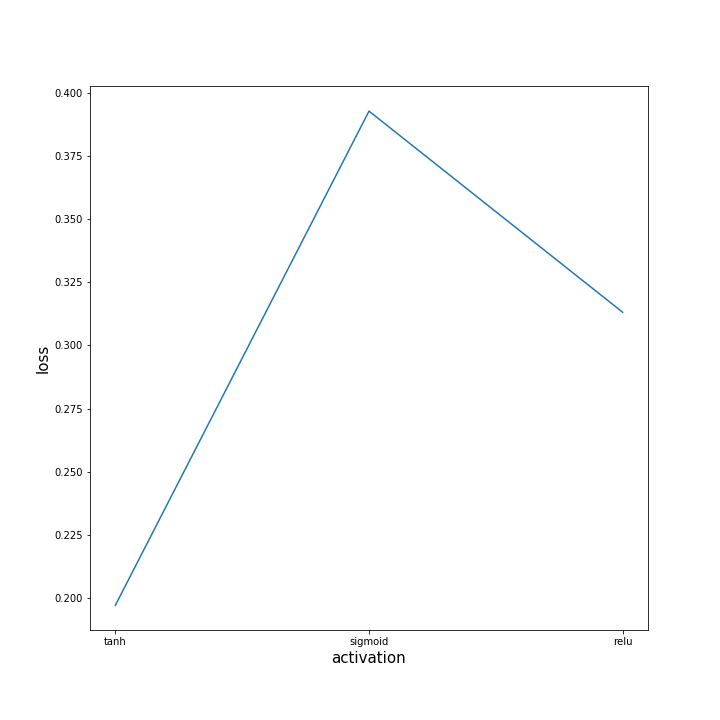
\includegraphics[width=0.45\textwidth]{perceptron_activation_search}
     }
     \caption{Перебор гиперпараметров}
     \label{fig:multi_perceptron_search}
\end{figure}
На рисунке \ref{fig:multi_perceptron_search} изображены графики значений функций ошибки в зависимости от параметров сети. Из графиков можно сделать вывод, что перебор гиперпараметров сети не даёт существенных улучшений качества предсказания сети на смещённой выборке.
\par
Большая часть публикаций по моделированию объектов управления многослойным перцептроном относится к 90-м годам XX века, и в основном в них, как например в \cite{fc90} и в \cite{fc90_2} многослойный перцептрон моделирует сложный нелинейный объект, при этом эксперименты с возможной экстраполяцией не проводятся.
\chapter{Реккурентная сеть из lstm ячеек}
\section{Структура сети}
\par
\begin{figure}[h]
\centering
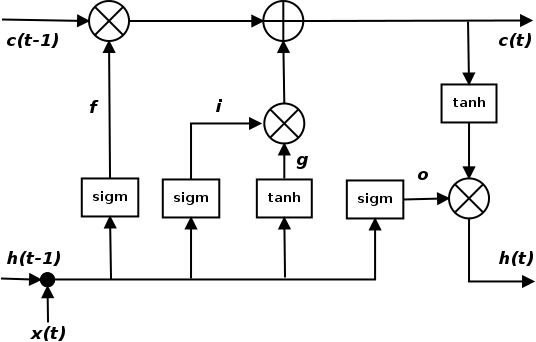
\includegraphics[width=0.5\textwidth]{lstm_cell}
\caption{Устройство lstm ячейки.}
\label{fig:lstm_cell}
\end{figure}
На рисунке \ref{fig:lstm_cell} схематично изображено устройство lstm ячейки. Из lstm ячеек составляют реккурентные сети, которые работают по принципу прогона одной и той же сети по участком входных данных фиксированной длины, при этом длина полного вектора входных может иметь любую длину. Между участками сеть передаёт так называемые векторы \textit{внутреннего состояния}, которые позволяют более явно учитывать зависимость входных значений в конкретной позиции от входных значений в предыдущих позициях. Реккурентные сети также как и многослойный перецептрон обучаются методом стохастического градиентного спуска, при этом градиент считается с помощью метода обратного распространения ошибки d раз, где d --- глубина рекурсии (для рассчёта рекурсия \textit{"<разворачивается">}, и сеть представляется как многослойная с повторяющимися весами), и усредняется по всем значениям. Для предсказания выходных значений в конкретной позиции обычно используется вектор внутреннего состояния, опционально пропущенный через линейнный слой и/или функцию softmax.
\par
Главное преимущество lstm ячейки состоит в использовании допольнительного \textit{вектора памяти}, который вычисляется независимо от вектора внутреннего состояния, сеть обучается \textit{запоминать} или \textit{забывать} определенную долю вектора памяти в зависимости от текущих входных данных, и это позволяет сети болле гибко воспроизводить зависимости внутри входной последовательности, и как следствие давать более точные (в сравнении с простейшей реккурентной сетью) предсказания. 
\section{Код и схема модели}
\par
\begin{figure}[h]
\centering
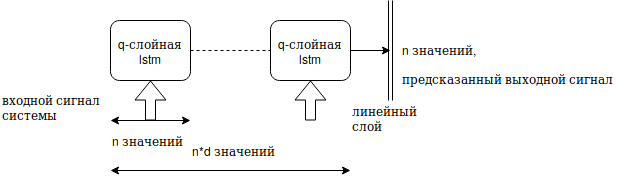
\includegraphics[width=0.9\textwidth]{rnn}
\caption{Использованная для экспериментов архитектура.}
\label{fig:lstm_net}
\end{figure}
На рисунке \ref{fig:lstm_net} изображена использованная для экспериментов архитектура реккурентной сети. Гиперпараметры сети: размер входного вектора lstm ячейки n; число внутренних слоёв ячейки q; максимальная глубина рекурсии d. В экспериментах на вход сети подавался вектор входного сигнала, кратный n, и сеть обучалась предсказывать выход объекта управления в последние n моментов времени. Реккурентные сети позволяют работать с последовательностями варьирующейся длины, поэтому в обучающую выборку входили векторы длины $1*n...d*n$, однако б\'oльшая часть обучающей выборки состояла из векторов длины $d*n$ для лучшего предсказания на таких данных. Такая сеть может быть реализована на языке python с использованием библиотеки pytorch:
\pagebreak
\begin{verbatim}
class ControlLSTMInputs(nn.Module):
    def __init__(self, window_size, layer_input_size,
        hidden_size, output_size, num_layers=2
        ):
        
        assert window_size % layer_input_size == 0
        super().__init__()
        self.reccurency = window_size // layer_input_size
        self.layer_input_size = layer_input_size
        
        self.layers = nn.ModuleList()
        self.layers.append(
            nn.LSTM(
                input_size=layer_input_size,
                hidden_size=hidden_size,
                num_layers=num_layers
            )
        )
        self.layers.append(nn.Linear(hidden_size, output_size))

    def forward(self, system_input_signal):
        hidden, _ = self.layers[0](system_input_signal.view(
            -1, self.reccurency, self.layer_input_size
        ).transpose(0, 1))
        last_hidden = hidden[-1, :, :]
        return self.layers[1](last_hidden)
\end{verbatim}
\par
Сеть обучалась с использованием среднеквадратичной ошибки в качестве функции ошибки.
\pagebreak
\section{Эксперименты}
\par
\begin{figure}[h]
\centering
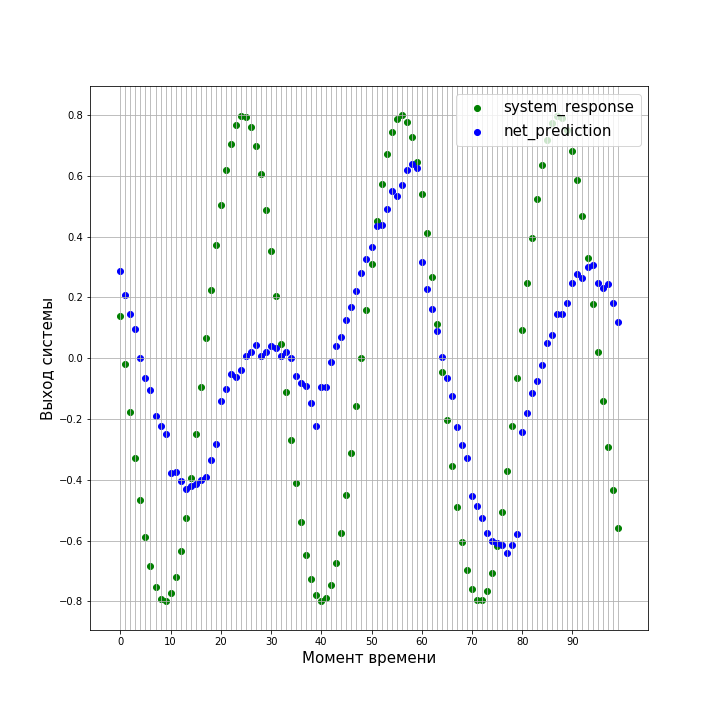
\includegraphics[width=0.9\textwidth]{rnn_prediction_shifted}
\caption{Предсказание при частоте 0.2~Гц.}
\label{fig:lstm_prediction_shifted}
\end{figure}
Графики предсказания сети на несмёщённой выборке выглядят абсолютно аналогично рисунку \ref{fig:multi_prediction} (предсказние практически идеально), поэтому они здесь не приведены. Гораздо интереснее выглядит изображённое на рисунке \ref{fig:lstm_prediction_shifted} предсказание выхода системы сетью, обученной на входных и выходных данных, полученных при подаче на вход системы сигналов из диапазона частот [0.05~Гц, 0.1~Гц], при подаче на вход сигнала с частотой 0.2~Гц. Пусть сеть не предсказывает достаточно релевантных данных, предсказание не выглядит как абсолютно не коррелирующее с реальными данными, и это подтверждается среднеквадратичной ошибкой при подаче сигналов со случайной частотой из равномерного распределения [0.1~Гц, 0.2~Гц], которая уменьшается в примерно в 3 раза: $0.06511564044169972$. Реккурентная сеть очевидно обладает лучшей способностью к экстраполяции поведения объекта управления. Хотя задача предсказания на смещённой выборке не всегда корректна, качество предсказния сети позволяет делать выводы о преимуществах реккурентной сети над многослойным перецептроном. 
\par
\begin{figure}[h]
\centering
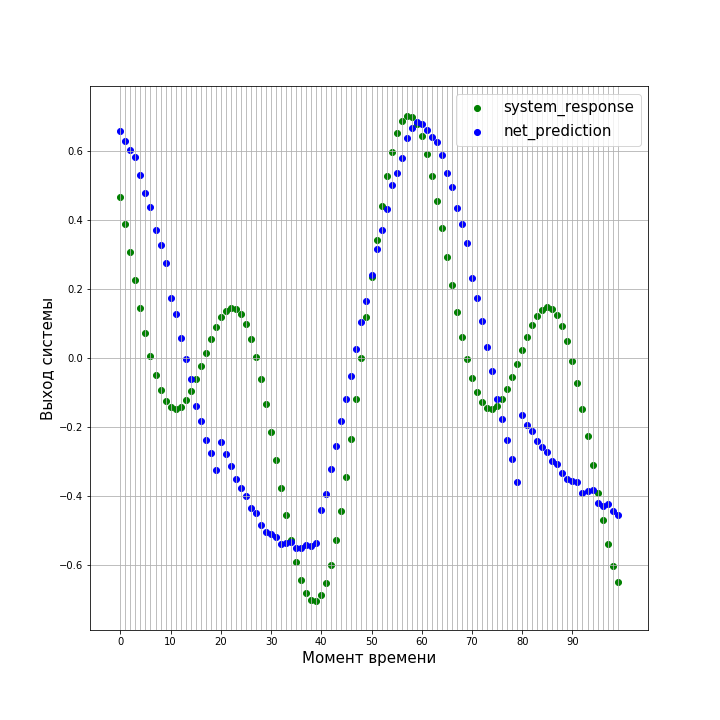
\includegraphics[width=0.9\textwidth]{rnn_prediction_mix}
\caption{Предсказание при синале из смеси 0.2~Гц и 0.1~Гц.}
\label{fig:lstm_prediction_mix}
\end{figure}
На рисунке \ref{fig:lstm_prediction_mix} изображено предсказание сети при подаче на вход смеси синусов с частотами 0.1~Гц и 0.2~Гц (обучение на тех же сигналах со случайной частотой из [0.05~Гц, 0.1~Гц]). Среднеквадратичная ошибка при подаче смеси сигнала со случайной частотой из [0.05~Гц, 0.1~Гц] с сигналом со случайной частотой из [0.1~Гц, 0.2~Гц]: $0.020396024022273196$. Можно сделать вывод, что подача сигнала с структурой, несколько отличающейся от структуры сигналов обучающей выборки, не влият негативно на предсказание сети.
\par
\begin{figure}[h]
\centering
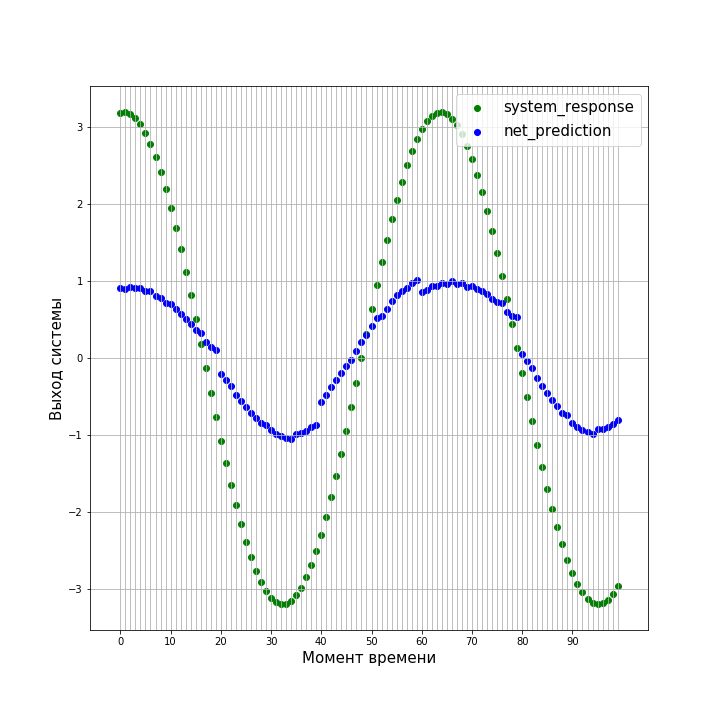
\includegraphics[width=0.9\textwidth]{rnn_prediction_high_magnitude}
\caption{Предсказание при увеличенной в 2 раза амплитуде входного сигнала.}
\label{fig:lstm_prediction_high_magnitude}
\end{figure}
На рисунке \ref{fig:lstm_prediction_high_magnitude} изображено предскзание сети при подаче на вход сети сигнала с частотой 0.1~Гц и амплитудой, увеличенной относительно амплитуды сигналов из обучающей выборки в 2 раза. Измерение среднеквадратичной ошибки на таких сигналах не имеет смысла, т. к. сеть в силу особенностей структуры не может воспроизводить сигналы с амплитудой больше 1, и среднеквадратичная ошибка всегда будет большой. Из графика можно заметить, что сеть не может корректно воспроизвести форму выходного сигнала, однако она способна воспроизвести его частоту. 
\par
\begin{figure}[!ht]
     \subfloat[Перебор размера скрытого слоя сети]{
         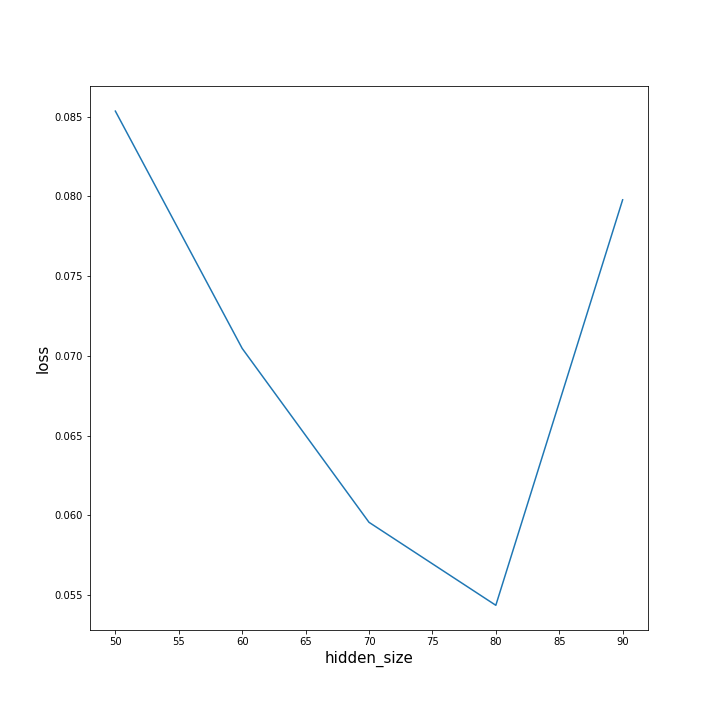
\includegraphics[width=0.45\textwidth]{lstm_hidden_size_search}
     }
     \hfill
     \subfloat[Перебор количества внутренних слоев]{
         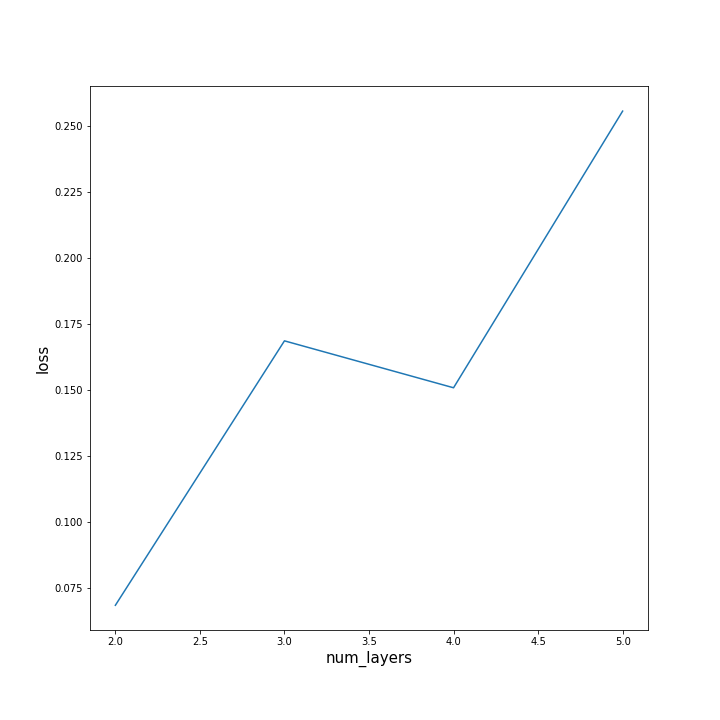
\includegraphics[width=0.45\textwidth]{lstm_num_layers_search}
     }
     \caption{Перебор гиперпараметров}
     \label{fig:lstm_search}
\end{figure}
На рисунке \ref{fig:lstm_search} изображены графики значений функции ошибки в зависимости от параметров сети. Из графиков можно сделать вывод, что перебор гиперпараметров сети позволяет добится некоторых улучшений качества предсказания, однако чрезмерное усложнение структуры сети (увеличение числа весов) ведёт к тому, что сеть переобучается, и качество предсказания на смещённой выборке падает. 
\par
В статьях, в которых используют lstm для моделирования и идентификации объектов управления, в \cite{deep_2017} и \cite{lstm_2017} моделируются сложные нелинейные объекты, и не делаются попытки экстраполяции, что вполне логично для сложных объектов.
\chapter{Реккурентная сеть из lstm ячеек, использующая данные выходов объекта управления при предсказании}
\section{Код и схема модели}
\par
\begin{figure}[h]
\centering
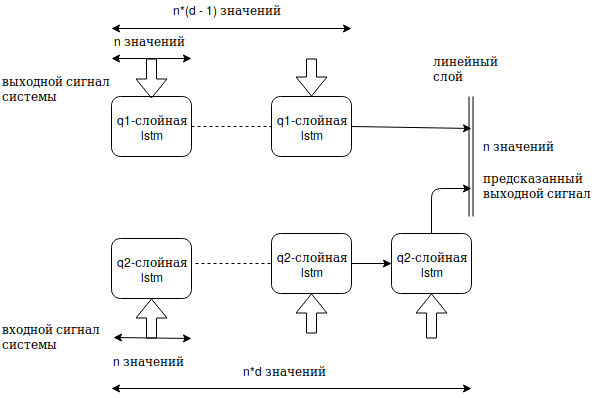
\includegraphics[width=0.8\textwidth]{updated_rnn}
\caption{Использованная для экспериментов архитектура.}
\label{fig:lstm_net_inputs}
\end{figure}
На рисунке \ref{fig:lstm_net_inputs} изображена архитектура сети, использовавшейся для третьего эксперимента. Эта сеть имеет много общего с сетью из предыдущего эксперимента, однако здесь присутствует сеть из lstm ячеек, которая учавствует в предсказании, и использует данные о выходе объекта управления в предыдущие моменты времени для предсказания. Гиперпараметры сети: число внутренних слоёв ячейки lstm q1, q2; размер входного слоя lstm ячейки n; максимальная глубина рекурсии d. При обучении сети используются данные реальных выходов объекта управления, а при предсказании предсказания сети в предыдущие моменты времени. Интуитивно такое различие входных данных при обучении и при предсказании должно негативно влиять на качество, однако, как видно из экспериментов, это не так. Идея использования ранее предсказанных целевых значений не нова, и так же широко применяется в обработке естественных языков, одной из областей с широким использованием реккурентных сетей и lstm. Использование предсказаний как входов для задач идентификации систем управления можно найти в статье \cite{lstm_2017}. Такая сеть может быть реализована на языке python  с использованием библиотеки pytorch:
\begin{verbatim}
class ControlLSTMInputsOutputs(nn.Module):
    def __init__(
        self,
        window_size,
        layer_input_size,
        hidden_size,
        output_size,
        num_layers=2
        ):
        assert window_size % layer_input_size == 0
        super().__init__()
        self.layer_input_size = layer_input_size
        self.reccurency_depth = window_size // layer_input_size
        self.hidden_size = hidden_size

        self.input_processing_cell = torch.nn.LSTM(
            input_size=layer_input_size,
            hidden_size=hidden_size,
            num_layers=num_layers
        )
        self.output_processing_cell = torch.nn.LSTM(
            input_size=layer_input_size,
            hidden_size=hidden_size,
            num_layers=num_layers
        )
        self.output_layer = (torch.nn.Linear(hidden_size * 2, output_size))

    def forward(self, system_input_signal, system_output_signal=None):
        assert system_output_signal is not None or \
               system_input_signal.size()[-1] == self.layer_input_size

        input_processing_hidden, _ = self.input_processing_cell(
            system_input_signal.view(
                # <batch_size>, <reccurency depth>, <one lstm cell input size>
                -1,
                system_input_signal.size()[-1] // self.layer_input_size,
                self.layer_input_size
                # transposing because view 
                # is incorrect if passing required shape to view directly
            ).transpose(0, 1)
        )
        if system_output_signal is not None:
            output_processing_hidden, _ = self.output_processing_cell(
                system_output_signal.view(
                    # <batch_size>, <reccurency depth>, <one lstm cell input size>
                    -1,
                    system_output_signal.size()[-1] // self.layer_input_size,
                    self.layer_input_size
                    # transposing because view 
                    # is incorrect if passing required shape to view directly
                ).transpose(0, 1)
            )
        else:
            output_processing_hidden = torch.zeros(input_processing_hidden.size())

        last_hidden = torch.cat((input_processing_hidden[-1, :, :],
            output_processing_hidden[-1, :, :]), -1)

        return self.output_layer(last_hidden)

\end{verbatim}
\par
Сеть обучалась с использованием среднеквадратичной ошибки в качестве функции ошибки.
\pagebreak
\section{Эксперименты}
\par
\begin{figure}[h]
\centering
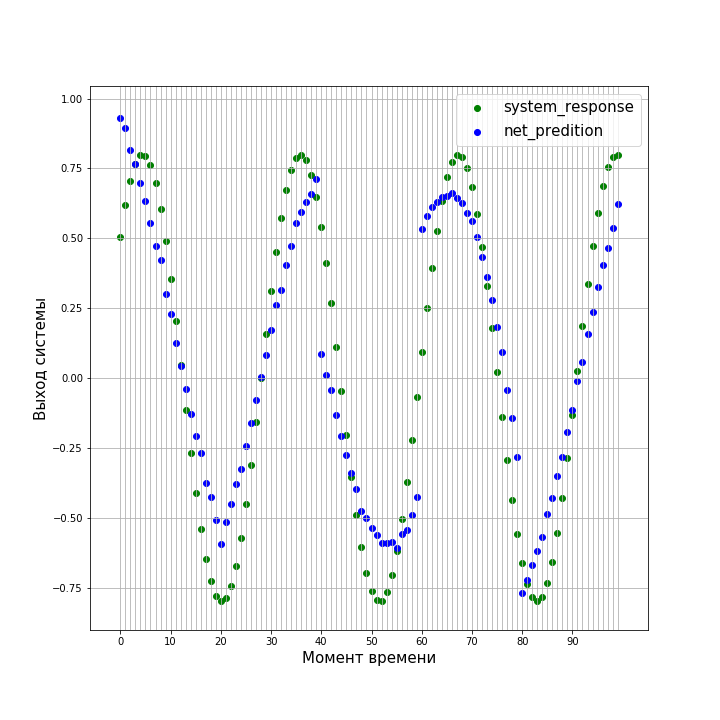
\includegraphics[width=0.9\textwidth]{rnn_2_prediction_shifted}
\caption{Предсказание при частоте 0.2~Гц.}
\label{fig:lstm_2_prediction_shifted}
\end{figure}
Как и прежде, на данных, аналогичных обучающей выборке, сеть предсказывает выход объекта управления практически идеально, поэтому график опускается. На рисунке \ref{fig:lstm_2_prediction_shifted} изображено предсказание выхода системы сетью, обученной на входных и выходных данных, полученных при подаче на вход системы сигналов из диапазона частот [0.05~Гц, 0.1~Гц], при подаче на вход сигнала с частотой 0.2~Гц. В сравнении с предыдущим экспериментом явно заметен прогресс, и это подтверждается значением среднеквадратичной ошибки при подаче на вход сети сигналов со случайной частотой из [0.1~Гц, 0.2~Гц], она равна: $0.012449543755501509$, в сравнении с предыдущим экспериментом это улучшение практически в 5 раз. Это позволяет сделать вывод о том, что использование данных о выходе сети однозначно улучшает предсказание.
\par
\begin{figure}[h]
\centering
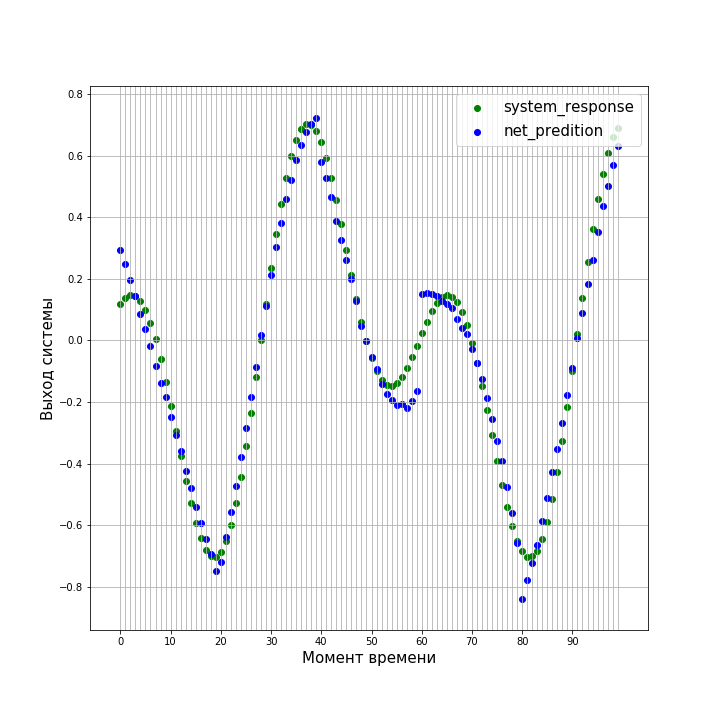
\includegraphics[width=0.9\textwidth]{rnn_2_prediction_mix}
\caption{Предсказание при синале из смеси 0.2~Гц и 0.1~Гц.}
\label{fig:lstm_2_prediction_mix}
\end{figure}
На рисунке \ref{fig:lstm_2_prediction_mix} изображено предсказание сети при подаче на вход смеси сигнала с частотой 0.1~Гц с сигналом с частотой 0.2~Гц. Как и для предыдущего случая, сеть использующая данные о выходном сигнале объекта управления предсказывает очевидно лучше сети, которая не использует данные о выходе. Это подтверждается среднеквадратичной ошибкой, она равна: $ 0.0014647390705067665$.
\pagebreak
\par
\begin{figure}[!ht]
     \subfloat[Перебор размера скрытого слоя сети]{
         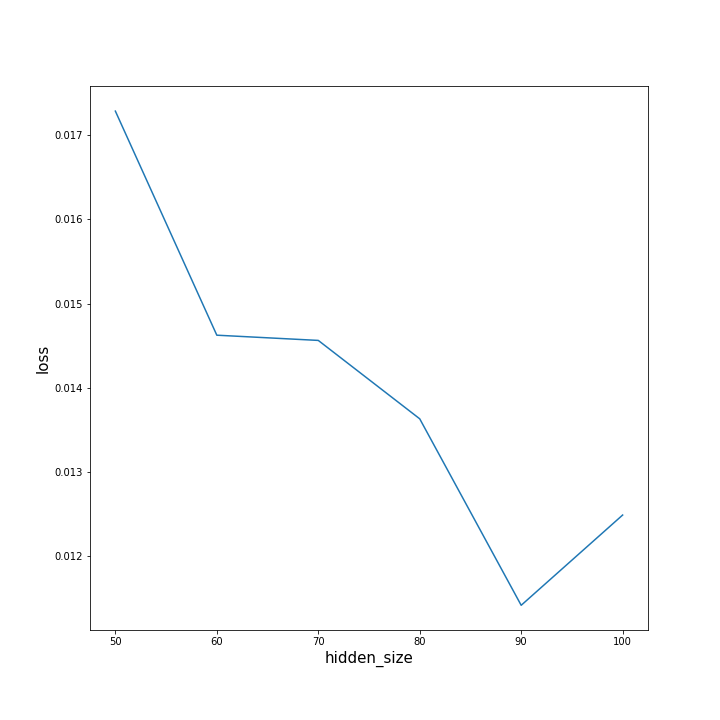
\includegraphics[width=0.45\textwidth]{lstm_2_hidden_size_search}
     }
     \hfill
     \subfloat[Перебор количества внутренних слоев]{
         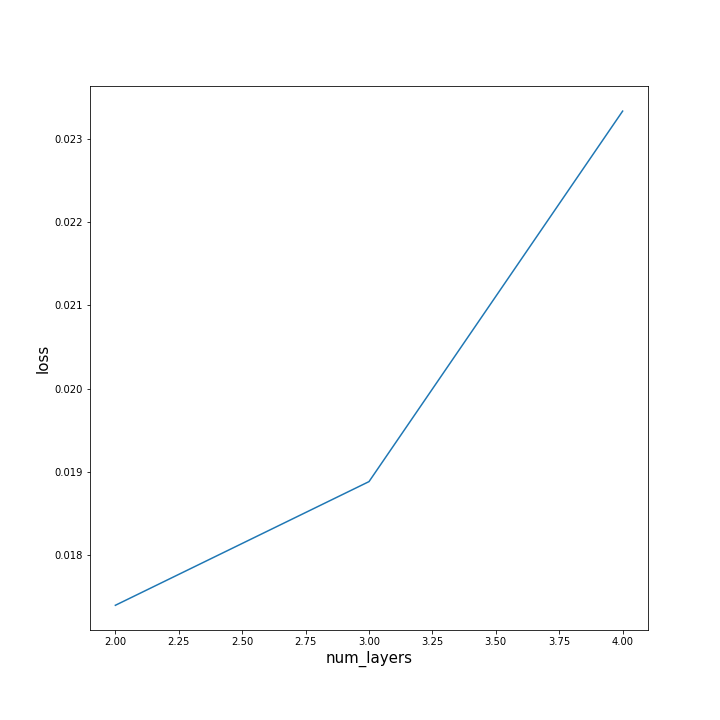
\includegraphics[width=0.45\textwidth]{lstm_2_num_layers_search}
     }
     \caption{Перебор гиперпараметров}
     \label{fig:lstm_2_search}
\end{figure}
На рисунке \ref{fig:lstm_2_search} изображены графики значений функций ошибки в зависимости от значений гиперпараметров сети. Как и прежде перебор гиперпараметров позволяет добится некоторых улучшений, но чрезмерное увеличение числа весов сети ведёт к переобучению и, как следствие, падению качества предсказания на смещённой выборке. 
\par В статье \cite{lstm_2017} сеть, использующая входы используется для моделирования сложного нелинейного объекта, и, как и прежде, не делается попыток экстраполяции.
\chapter{Заключение}
\par
В ходе работы был проведён сравнительный анализ качества моделирования объекта управления для задачи идентификации нейронными сетями с различными архитектурами, из экспериментов можно сделать выводы:\\
\begin{itemize}
\item Реккурентная сеть основанная на lstm ячейках, использующая данные входов и выходов объекта управления для  предсказания выхода объекта управления, моделирует объект управления однозначно наилучшим образом среди всех рассмотреных сетей.
\item Определён примерный вектор дальнейшего улучшения оптимальной архитектуры сети для решения задач идентификации объектов управления, а именно: сеть долна иметь реккурентную архитектуру; сеть должна использовать данные о выходах системы управления в предыдущие моменты времени или собственные предсказания как входы; сеть должна состоять из lstm или сопоставимых по качеству в различных задачах ячеек реккурентной сети.
\item Сеть не должна иметь чрезмерно большое, т. е. неадекватное сложности системы число параметров во избежание переобучения на данных обучающей выборки. Число параметров можно оценивать эмпирически с помощью обучения на определённой части обучающей выборки и проверки качества предсказания на другой её части.
\end{itemize}
\begin{thebibliography}{1}
\bibitem{fc90} KUMPATI S. NARENDRA FELLOW, IEEE. AND KANNAN  PARTHASARATHY, Identification and control of dynamical systems using neural networks, 1990. https://ieeexplore.ieee.org/abstract/document/80202
\bibitem{fc90_2} Neural Networks for System Identification. S. Reynold Chu, Rahmat Shoureshi, and Manoel Tenorio, 1990. https://ieeexplore.ieee.org/abstract/document/55121
\bibitem{deep_2017} Nonlinear Systems Identification Using Deep Dynamic Neural Networks. Olalekan Ogunmolu, Xuejun Gu, Steve Jiang, and Nicholas Gans, 2017. https://arxiv.org/abs/1610.01439
\bibitem{lstm_2017} A new concept using LSTM Neural Networks for dynamic system identification. Yu Wang, 2017. https://ieeexplore.ieee.org/abstract/document/7963782
\bibitem{source_code} $https://github.com/antosiv/study\_progs/tree/master/jupyter/diploma$
\end{thebibliography}
\end{flushleft}
\end{document}
